\setlength{\columnsep}{3pt}
\begin{flushleft}
	\bigskip
	\begin{itemize}
		\item Each file contains metadata \& an identification number, called an inode number.
		\item The inode number refers to the \textbf{physical file \& the data stored in a particular location}.
		\item An inode number contains files metadata as shown below:
			\begin{figure}[h!]
				\centering
				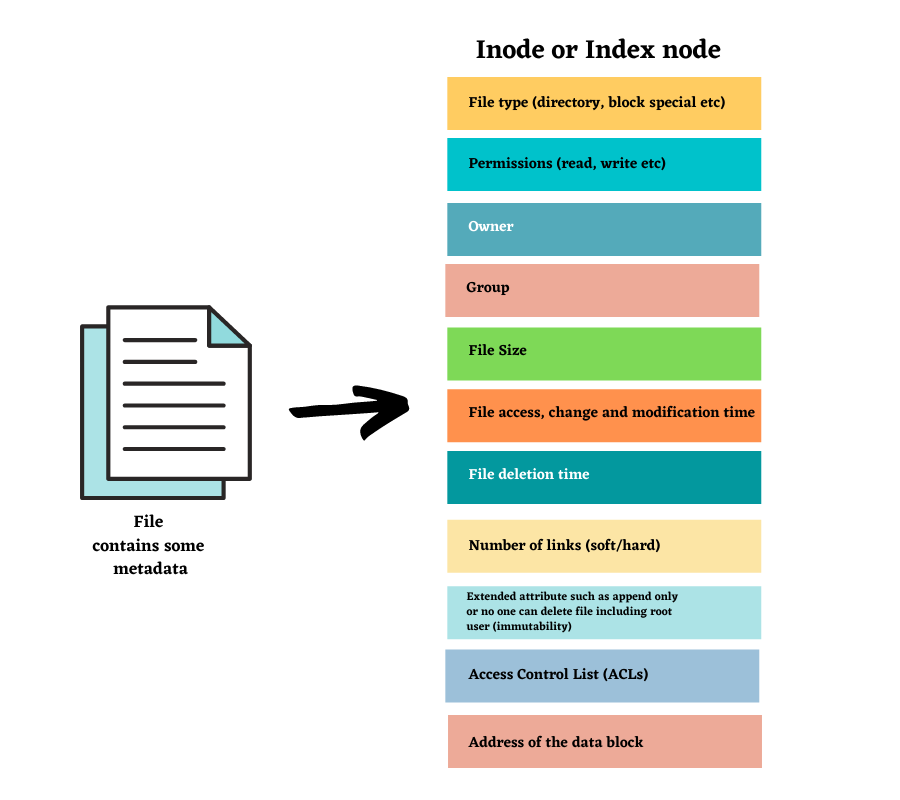
\includegraphics[scale=.6]{content/chapter10/images/metadata.png}
				\caption{File metadata}
				\label{fig:File_attributes}
			\end{figure}
		
	\end{itemize}
	
\end{flushleft}

\newpage

